\section{Innledning}

%I innledningen skal du plassere deg i fagfeltet og vise at du har kjennskap til tidligere forskning. Innledningen skal gjøre rede for hva vi vet og hva vi ikke vet om feltet.

%Dette gjør du ved å presentere:

%et problem eller et fenomen du skal studere

\begin{figure} 
\begin{center} 
\includegraphics[scale=0.05]{../data/train/atlantic_cod/fish_2690}
\includegraphics[scale=0.05]{../data/train/atlantic_cod/fish_6040}
\includegraphics[scale=0.05]{../data/train/atlantic_cod/fish_8540}
\includegraphics[scale=0.05]{../data/train/atlantic_cod/fish_10440}
\includegraphics[scale=0.05]{../data/train/atlantic_cod/fish_4940}
\includegraphics[scale=0.05]{../data/train/atlantic_cod/fish_5740}
\caption{\small \sl Figuren viser eksempelbilder fra en video av en lagringsmerd med torsk. Disse bildene er en del av datasettet anvendt for deteksjon av torsk og sei. \label{fig:data}} 
\end{center} 
\end{figure} 

Her presenteres automatisk fiskedeteksjon av torsk og sei fra bilder tatt med undervannskameraer. Modellen er trent opp på fisk fra merder brukt til fiskeoppdrett og lagring. Se figur \ref{fig:data}.

Dette arbeidet er viktig for å forstå omfanget av torsk og sei som trekker til oppdrettsanlegg og spiser oppdrettsfôr fra under merdene. Forskere, samt fiskere og oppdrettsnæringen, ønsker å samle informasjon om villfisk som spiser oppdrettsfôr, fôret kan til forskjellige tider inneholde medisinrester. Manuell analyse av data fra undervannskameraer er tidskrevende, dessuten kan det kreve ekspertkunnskap om forskjellige fiskearter. Dette gjør det veldig vanskelig å gjennomføre et større datainnsamlingsprosjekt. Til tross for vanskelighetene så er slike analyser viktige. Kunnskap om de marine økosystemene, og effekten oppdrettsnæringen har på mattrygghet og kvalitet av villfisk, berører fiskere og befolkningen som spiser norsk fisk. Derfor er verktøy som gjør automatisk videoanalyse nødvendig, og bør utvikles for å støtte forskere i arbeidet deres.

Dette prosjektet er gjort i samarbeid med Nofima som en del av Sameksistens prosjektet \cite{Robertsen 2020}. Dataprogrammet som har blitt utviklet for denne oppgaven kan ta imot undervannsvideo med høy oppløsning og telle antall norsk torsk og sei fortløpende.

%bakgrunnen for valg av tema
%problemstillingen eller hypotesene du skal undersøke
%På slutten av introduksjonen kan du også si noe om hvordan du har tenkt å strukturere resten av oppgaven, som en kort leserguide.

%Et tips er å begynne å skrive på innledningen tidlig, slik at den kan gi retning for det videre arbeidet ditt. Så går du heller over innledningen igjen på slutten for å skrive den helt ferdig. Da får du en innledning som har god sammenheng med resten av teksten.

\subsection{Bakgrunn}

\begin{figure} 
\begin{center} 
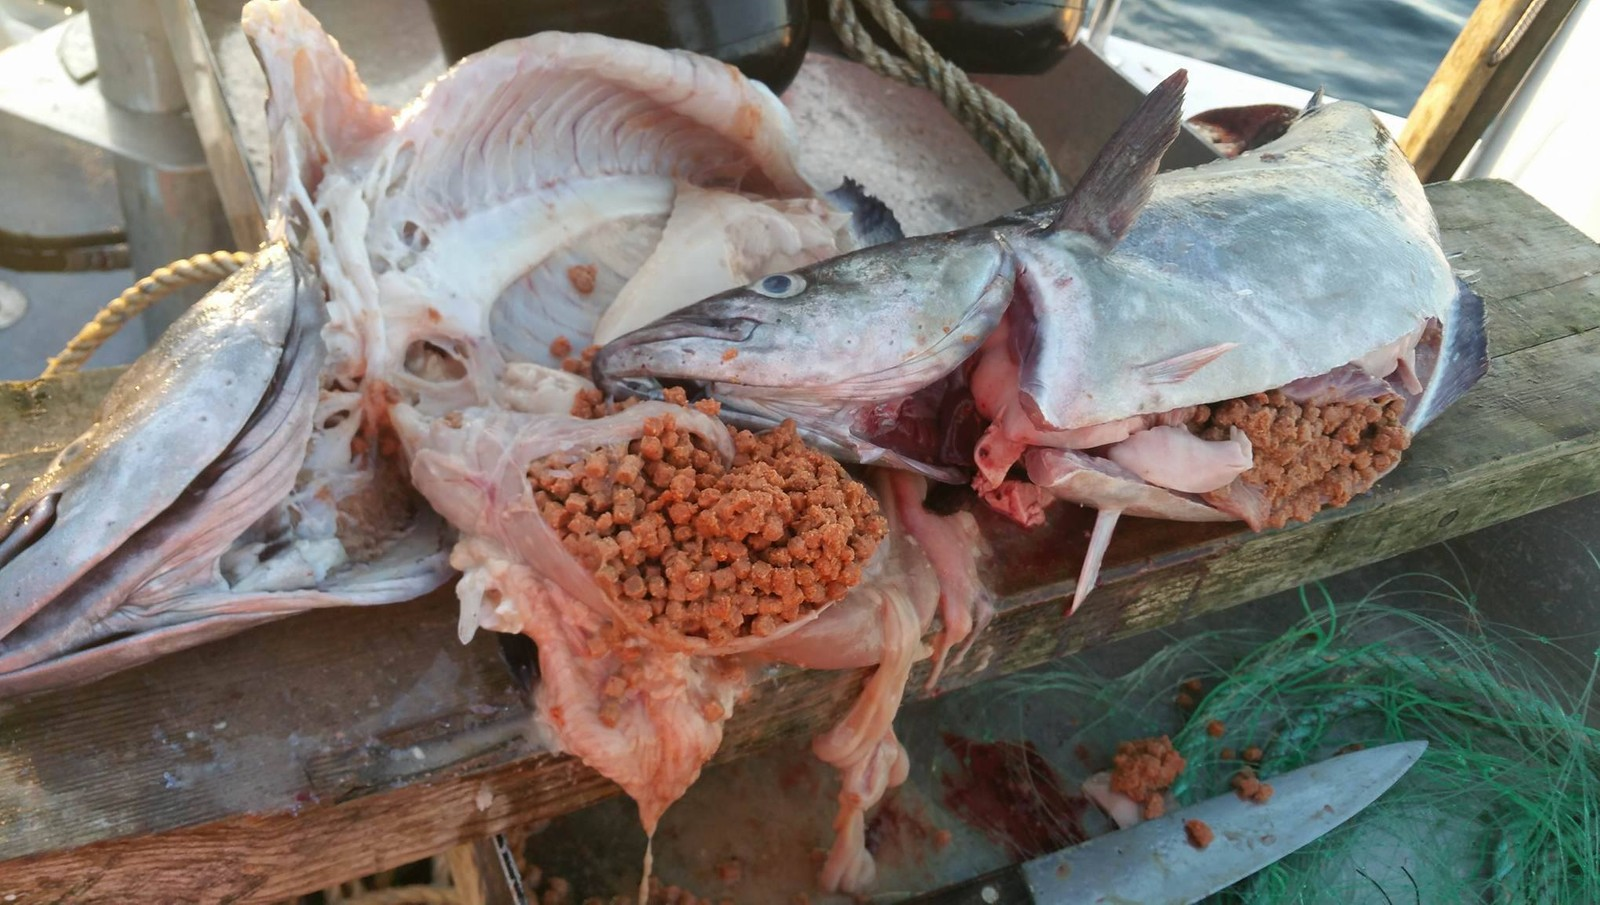
\includegraphics[scale=0.2]{figures/oppdrettfor}
\caption{\small \sl Figuren viser et eksempel av ``pellets-fisken''. Det lukter ekkelt og det er forferdelig å sløye en fôrsprengt fisk, ifølge flere fiskere som har vært i kontakt med NRK \cite{Trana m.fl. 2019}. Seien har vært under merdene, da blir den full av pellets. Fôrsprengt fisk er unaturlig, hode blir for liten og kroppen for stor. Dette har pågått i mange år. Likevel blir fisken omsatt, fiskere får levert slik fisk til enkelte fiskebruk. \cite{Angell og Ekanger 2017} \label{fig:oppdrettfor}} 
\end{center} 
\end{figure} 

\begin{figure}
\begin{center} 
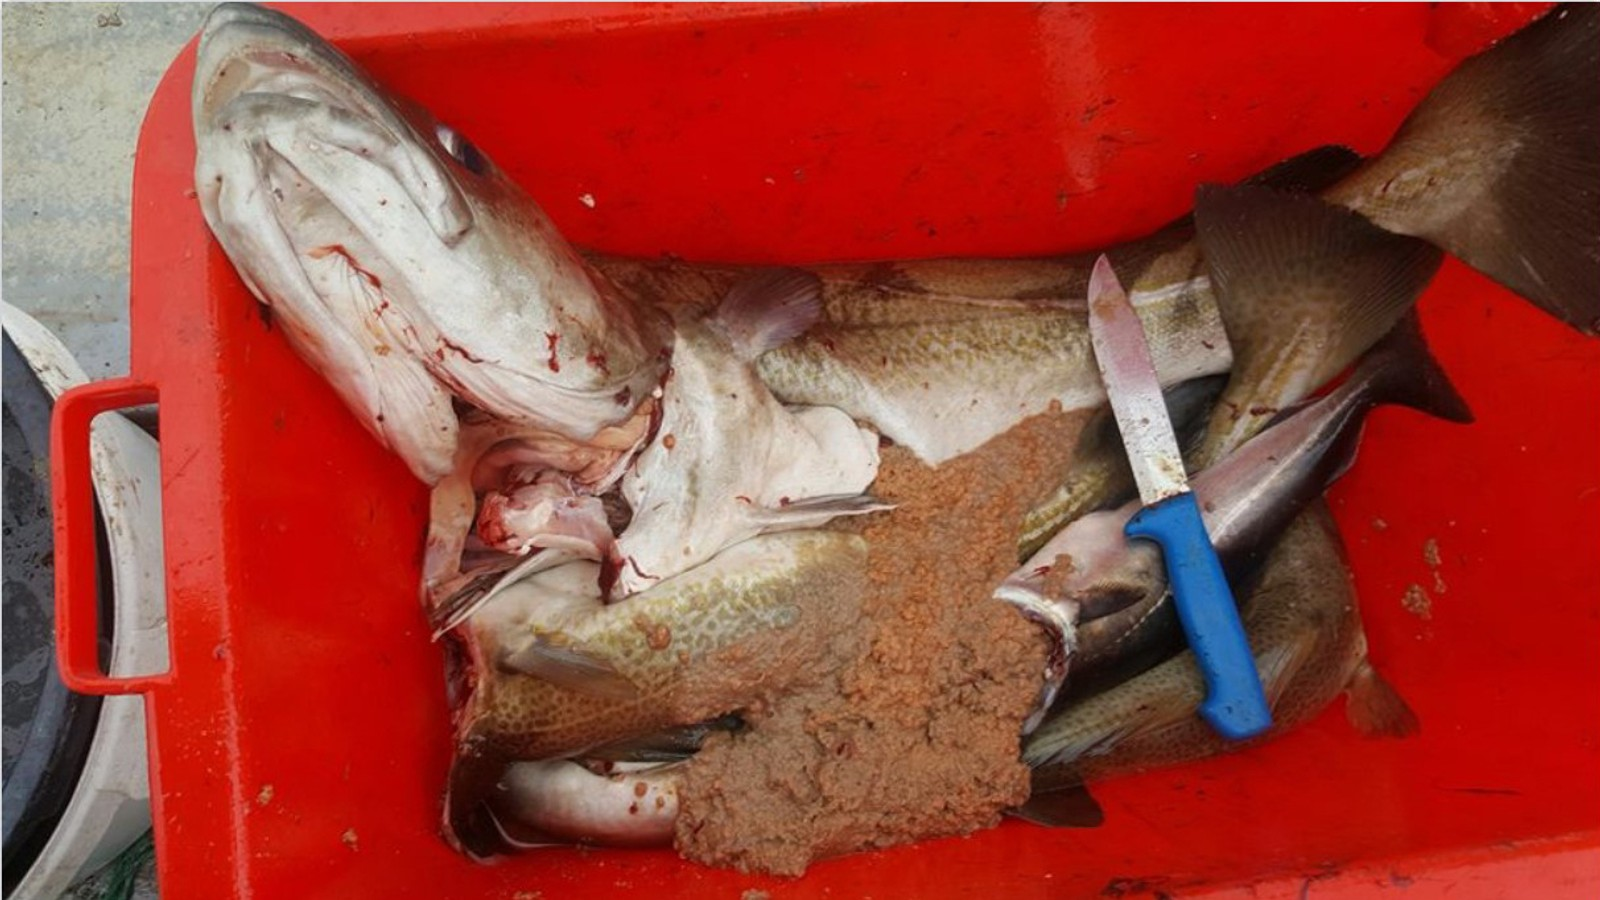
\includegraphics[scale=0.2]{figures/forsprengt}
\caption{\small \sl Figuren viser et eksempel av fôrsprengt fisk. Det lukter ekkelt og det er forferdelig å sløye en fôrsprengt fisk, ifølge flere fiskere som har vært i kontakt med NRK. Foto: Arnold Jensen. \cite{Trana m.fl. 2019} \label{fig:forsprengt}} 
\end{center} 
\end{figure} 

Kystfiskere hevder villfisken får i seg så mye laksefôr at fiskeplassene blir ødelagt. ``Litt overraskende utspill'' svarer oppdrettsbransjen. Fisker Tor Inge Larsen i Brønnøysund sa til NRK i 2018 at han fortviler over det han mener er dårligere kvalitet hos fisken han fanger. Han sa han kan knapt huske sist han fikk en sei om bord i båten uten at den hadde pellets fra lakseoppdrett i magen. Han hevder fiskerne har blitt frastjålet fiskeområder på høylys dag, og mener fiskefeltene nært Brønnøysund på Sør-Helgeland i Nordland har fått betydelig lavere kvalitet på grunn av oppdrettsanleggene. \cite{Olsen m.fl. 2018}

Johnny Eliassen som er bosatt på Reinøya i Troms, Karlsøy kommune, fortalte til NRK at han hadde tidligere engasjert seg i saken for å hindre at kystområdet ble lokasjon for oppdrettsanlegg. Det ble allikevel åpnet et oppdrettsanlegg mai 2017 i fjorden på Reinøya, og det hevder de lokale fiskerne at de har merket. De har fisket ``pelletstorsk'',  torsk med magen full av pellets, selv over en kilometer unna anlegget. Oppdrettere reklamerer oppdrettsfisk som den absolutte beste fisken. Eliassen kunne ikke tenke seg er at det virkelig er tilfelle, for lukten og konsistensen på fisken gjør den uspiselig i hans øyne. \cite{Jakobsen 2017}

Men fiskerne og forskerne har vært uenige om hvorvidt pellets fra lakseoppdrett påvirker kvaliteten av vill fisk som spiser den. Det er forsket relativt lite på hvordan oppdrett påvirker villfisk. Seniorrådgiver Bjørn-Steinar Sæther fra Nofima ga ut en artikkel i 2017 der han mener seien som hadde spist oppdrettsfôr får en litt bløtere og noe mer spaltet muskel enn annen sei, men den var fortsatt stort sett innenfor kategorien god kvalitet. \cite{Saether 2017}

Kommunikasjonsdirektør Are Kvistad i Sjømat Norge er litt overrasket over utspillet fra fiskeren på Helgeland. Han mener laksepellets ikke utgjør noen fare for villfisk. ``Det er et fiskefôr som blir sjekket av myndighetene, og er et trygt og næringsrikt fôr som også er trygt for villfisk'', sa Kvistad til NRK i 2018. Kvistad mente det også er i oppdretternes interesse, både økonomisk og utslippsmessig, å redusere fôringen av oppdrettslaksen slik at den kun får den maten den trenger. \cite{Olsen m.fl. 2018}

Vinteren 2018 rømte 52 000 laks fra Marine Harvests oppdrettsanlegg i Nærøy kommune i Trøndelag. Ifølge Namdalsavisa inneholdt laksen medisiner mot innvollsorm. Mattilsynet gikk ut og sa at det var trygt å spise fisken, men at den ikke kunne omsettes videre. \cite{nrk 2018}

Den rømte laksen hadde blitt gitt medisinfôr med praziquantel og skulle være i karantene i 14 dager. For fiskere, slik som Arnold Jensen, er denne informasjonen skremmende. Jensen er medlem av Naturvernforbundets fiske- og oppdrettsutvalg. Han ønsker at mattryggheten til villfisk som beiter ved oppdrettsanleggene skal kontrolleres. Se figur \ref{fig:oppdrettfor} og \ref{fig:forsprengt}. \cite{Christensen 2019}

I 2019 kom ``pellets-fisken'' i medienes søkelys igjen, denne gangen var det fiskere i Lyngen kommune i Troms som slo alarm. Villfisk som hadde spist oppdrettsfôr som inneholdt medisin omsettes av fiskere i fjorden. De ønsker svar på om det kan være farlig for forbrukere. \cite{Trana m.fl. 2019}

\begin{figure} 
\begin{center} 
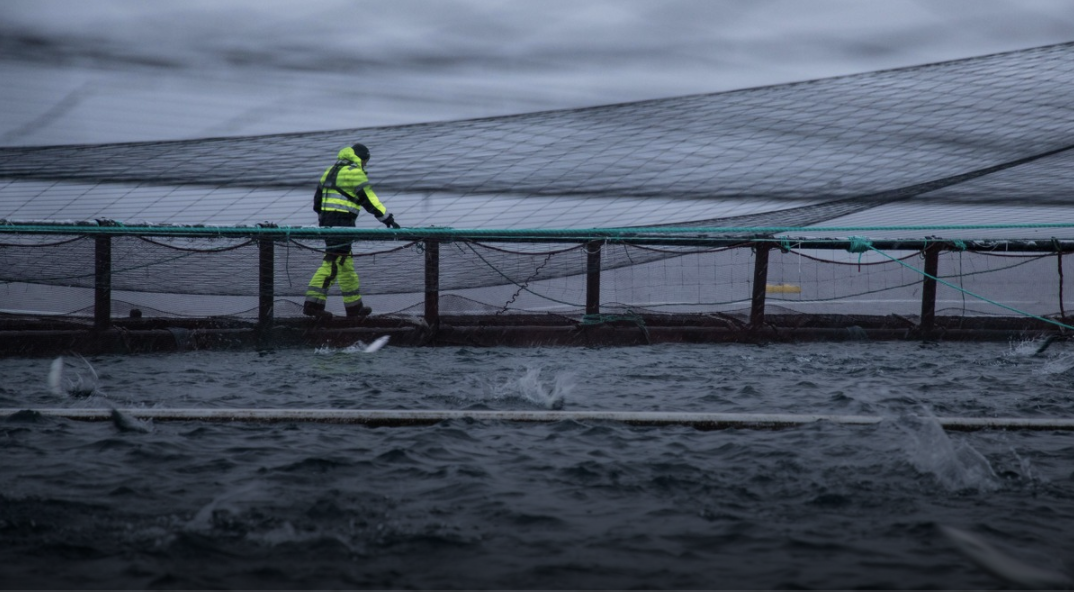
\includegraphics[scale=0.7]{figures/oppdrett}
\caption{\small \sl Figuren viser et oppdrettsanlegg. Fôret oppdrettsfisken mates med spises også av villfisk. Oppdrettsbransjen er i konflikt med fiskere som mener oppdrettsnæringen ødelegger fiskeplasser i fjordene med anlegg og reduserer kvaliteten til villfisk som spiser fôrpellets under merdene. \cite{Olsen m.fl. 2018} \label{fig:anlegg}} 
\end{center} 
\end{figure} 

Sjømatdivisjonen og Akvadivisjonen ved Nofima har en strategisk internsatsing som går ut på å samle kunnskap om sameksistens mellom ulike marine næringer og interesser, deriblant om hvordan man kan unngå konflikter mellom ulike interesser. Se figur \ref{fig:anlegg}. \cite{Robertsen 2020}

En av problemstillingene er sameksistens mellom fiskeri- og oppdrettsnæringene, og hvordan oppdrettsanlegg påvirker de nærliggende fiskeplassene. I den forbindelse er det interessant å kartlegge omfanget av hvitfisk som beiter på fôr fra oppdrettsanlegg. Dette er en problemstilling som har vært i fokus hos media etter at flere fiskere har fanget fôrsprengt torsk og sei i fjorder hvor det finnes oppdrettsanlegg. Det hevdes at denne fisken er av betydelig dårligere kvalitet og den kan ha fått i seg medisiner gjennom fôret som gjør at den kan være farlig å spise. \cite{Olsen 2019}

Det behøves kunnskap om hvor mange villfisk som trekker til oppdrettsanlegg, og under hvilke forhold, slik at man kan komme nærmere en løsning som kan dempe konflikten mellom disse to næringene. 

Målet med dette prosjektet var å utvikle et system som kan telle antall villfisk av ulike arter basert på en videostrøm fra et undervannskamera. Det er ønskelig å kunne vise resultatet som en fordeling av observasjoner over tid for hver art. 

\subsection{Kunstig intelligens}

\begin{figure} 
\begin{center} 
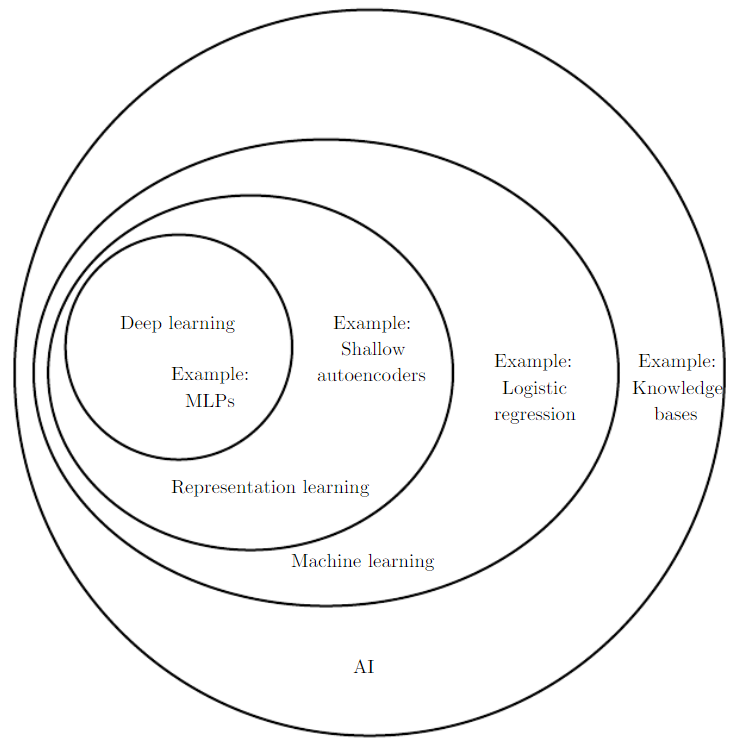
\includegraphics[scale=0.7]{figures/ai}
\caption{\small \sl Figuren viser et Venn diagram som viser at deep learning er en form for representativ læring, og det er igjen en form for maskinlæring. Maskinlæring er anvendt i mange, men ikke alle, de forskjellige metodene innenfor kunstig intelligens. Hver del av Venn diagrammet gir et eskempel av anvendelsen til teknolgien. \cite{Goodfellow m.fl. 2016 s. 9} \label{fig:ai}} 
\end{center} 
\end{figure} 

Tilbake på 1840-tallet, da programmering av datamaskiner ble oppfunnet, så spurte matematikere av den tiden seg selv om slike maskiner kunne bli intelligente, selv over hundre år før en datamaskin faktisk hadde blitt bygget (Lovelace 1842). I dag så har kunstig intelligens (KI) blitt et stort forskningsfelt med mange praktiske anvendelser og aktive forskningsprosjekter. Intelligent programvare automatiserer trivielt arbeid, forstår tale og kjenner igjen objekter i bilder, kan diagnosere pasienter innenfor medisin og hjelper forskere med grunnforskning. \cite{Goodfellow m.fl. 2016 s. 1}

Dette projektet beskriver maskiner som kan gi en tidsoversikt over torsk og sei fra en videostrøm. Den lærer konseptene en torsk eller sei består av, den lærer fra data. Maskinlæring, å la en maskin lære fra data, er kun en av metodene innenfor kunstig intelligens. Se figur \ref{fig:ai}. Kunstig intelligens har vært igjennom to ``vintre'', men de siste åtte årene har vært en ny gullalder for kunstig intelligens etter introduksjonen av AlexNet i 2012. \cite{Canziani m.fl. 2017 s. 1}

I begynnelsen så løste kunstig intelligens problemer, med fremragende hastighet, som var intellektuelt vanskelig for mennesker å løse, men relativt trivielle for datamaskiner. Problemene kunne beskrives formelt, med matematiske regler. Utfordringen med kunstig intelligens viste seg å være å løse problemer som var enkle for mennesker å utføre, men vanskelige for mennesker å beskrive formelt. Dette er problemer som vi løser intuitivt, som føles automatiske ut, slik som å forstå ordene til andre mennesker, ansiktene deres, og å kjenne igjen det en har sett tidligere i bilder. \cite{Goodfellow m.fl. 2016 s. 1}

Denne oppgaven handler om å finne løsninger på intuitive problemer. Løsningen er å la datamaskiner lære fra erfaringer og forstå verden ved å forstå konsepter, som kan igjen bli forstått med enda enklere konsepter. Denne samlingen av kunnskap fra erfaring som datamaskinene gjør seg selv, uten at et menneske formelt beskriver kunnskapen til maskinen, kan beskrives med en graf. Se figur \ref{fig:deep}. Ettersom denne grafen kan bestå av mange lag, den er dyp, så kalles denne formen for maskinlæring ``deep learning''. \cite{Goodfellow m.fl. 2016 s. 1}

%"Deep Learning" is a general term that usually refers to the use of neural networks with multiple layers that synthesize the way the human brain learns and makes decisions. A convolutional neural network is a kind of neural network that extracts features from matrices of numeric values (often images) by convolving multiple filters over the matrix values to apply weights and identify patterns, such as edges, corners, and so on in an image. The numeric representations of these patterns are then passed to a fully-connected neural network layer to map the features to specific classes. https://notebooks.azure.com/graememalcolmoutlook/projects/mlprimers/html/05a%20-%20Image%20Classification%20with%20a%20CNN%20(PyTorch).ipynb

\begin{figure} 
\begin{center} 
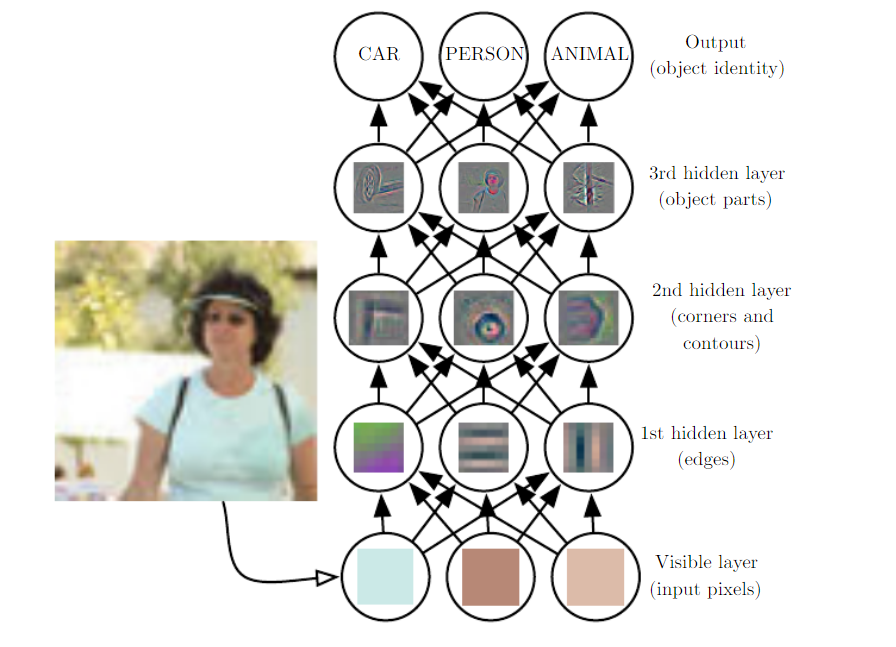
\includegraphics[scale=0.7]{figures/deep}
\caption{\small \sl Figuren viser en deep learning modell. Det er vanskelig for en datamaskin å forstå hva en matrise av sensorisk rådata er, slik som dette bilde representert som en samling pikselverdier, en matrise. Å lage en funksjon som tar inn piksler og gir ut en objektidentitet er svært komplisert. Å finne på en slik funksjon virker nærmest umulig om en takler problemet direkte. Deep learning løser vanskelighetene ved dele opp den kompliserte funksjonenen til en samling sammenkobledde funksjoner. Disse funksjonene kalles ofte for kunstige neuroner, kerneler eller filtere. Utmatningene fra kernelene i ett lag blir innmatningene til neste lag i modellen. Innmatningen til modellen, slik som et bilde, kalles for det synlige laget, ettersom den består av informasjon som vi mennesker kan forstå. Dette laget er etterfult av en serie med skjulte lag, ``hidden layers'', hvert lag henter ut mer og mer abstrakte erfaringer, ``features'', fra bildet. Disse lagene kalles for ``hidden'' ettersom verdiene i disse lagene finnes ikke i innmatningen til nettverket; modellen må selv bestemme hvilke konsepter som er nyttige for å beskrive sammenhengen i det synlige laget. Hvert lag danner forskjellig innsikt. Det første laget kan for eksempel lett gjenkjenne kantene i et bilde ved å sammenligne kontraster i bilde. Denne informasjonen sendes til det neste laget, et lag som finner kanter. Gitt det andre skjulte lagets beskrivelse av bilde, et bilde beskrevet med kanter, så kan objektdeteksjon bli mulig ved å sammenligne en samling kanter, konturer, med deler av kjente objekter. \cite{Goodfellow m.fl. 2016 s. 6} \label{fig:deep}} 
\end{center} 
\end{figure} 

%The difficulties faced by systems relying on hard-coded knowledge suggestthat AI systems need the ability to acquire their own knowledge, by extracting2
%CHAPTER 1. INTRODUCTIONpatterns from raw data. This capability is known asmachine learning. Theintroduction of machine learning enabled computers to tackle problems involvingknowledge of the real world and make decisions that appear subjective. A simplemachine learning algorithm calledlogistic regressioncan determine whether torecommend cesarean delivery (Mor-Yosef et al., 1990). A simple machine learningalgorithm called naive Bayes can separate legitimate e-mail from spam e-mail \cite{Goodfellow m.fl. 2020 s. 3}

%The performance of these simple machine learning algorithms depends heavilyon therepresentationof the data they are given. For example, when logisticregression is used to recommend cesarean delivery, the AI system does not examinethe patient directly. Instead, the doctor tells the system several pieces of relevantinformation, such as the presence or absence of a uterine scar. Each piece ofinformation included in the representation of the patient is known as afeature.Logistic regression learns how each of these features of the patient correlates withvarious outcomes. However, it cannot influence how features are defined in anyway. If logistic regression were given an MRI scan of the patient, rather thanthe doctor’s formalized report, it would not be able to make useful predictions.Individual pixels in an MRI scan have negligible correlation with any complicationsthat might occur during delivery. \cite{Goodfellow m.fl. 2020 s. 3}

%This dependence on representations is a general phenomenon that appearsthroughout computer science and even daily life. In computer science, operationssuch as searching a collection of data can proceed exponentially faster if the collec-tion is structured and indexed intelligently. People can easily perform arithmeticon Arabic numerals but find arithmetic on Roman numerals much more timeconsuming. It is not surprising that the choice of representation has an enormouseffect on the performance of machine learning algorithms. For a simple visualexample, see figure 1.1.

%Many artificial intelligence tasks can be solved by designing the right set offeatures to extract for that task, then providing these features to a simple machinelearning algorithm. For example, a useful feature for speaker identification fromsound is an estimate of the size of the speaker’s vocal tract. This feature gives astrong clue as to whether the speaker is a man, woman, or child.

%For many tasks, however, it is difficult to know what features should beextracted. For example, suppose that we would like to write a program to detectcars in photographs. We know that cars have wheels, so we might like to use thepresence of a wheel as a feature. Unfortunately, it is difficult to describe exactlywhat a wheel looks like in terms of pixel values. A wheel has a simple geometricshape, but its image may be complicated by shadows falling on the wheel, the sunglaring off the metal parts of the wheel, the fender of the car or an object in the foreground obscuring part of the wheel, and so on.

%One solution to this problem is to use machine learning to discover not onlythe mapping from representation to output but also the representation itself.This approach is known asrepresentation learning. Learned representationsoften result in much better performance than can be obtained with hand-designedrepresentations. They also enable AI systems to rapidly adapt to new tasks, withminimal human intervention. A representation learning algorithm can discover agood set of features for a simple task in minutes, or for a complex task in hours tomonths. Manually designing features for a complex task requires a great deal ofhuman time and effort; it can take decades for an entire community of researchers.

%The quintessential example of a representation learning algorithm is theau-toencoder. An autoencoder is the combination of anencoderfunction, whichconverts the input data into a different representation, and adecoderfunction,which converts the new representation back into the original format. Autoencodersare trained to preserve as much information as possible when an input is runthrough the encoder and then the decoder, but they are also trained to make thenew representation have various nice properties. Different kinds of autoencodersaim to achieve different kinds of properties.

%A major source of difficulty in many real-world artificial intelligence applicationsis that many of the factors of variation influence every single piece of data we areable to observe. The individual pixels in an image of a red car might be very closeto black at night. The shape of the car’s silhouette depends on the viewing angle.Most applications require us to disentangle the factors of variation and discard theones that we do not care about.

%Deep learningsolves this central problem in representation learning by intro-ducing representations that are expressed in terms of other, simpler representations.Deep learning enables the computer to build complex concepts out of simpler con-cepts. Figure 1.2 shows how a deep learning system can represent the concept ofan image of a person by combining simpler concepts, such as corners and contours,which are in turn defined in terms of edges.

%The quintessential example of a deep learning model is the feedforward deepnetwork, ormultilayer perceptron(MLP). A multilayer perceptron is just amathematical function mapping some set of input values to output values. Thefunction is formed by composing many simpler functions. We can think of eachapplication of a different mathematical function as providing a new representationof the input.

%Programvaren implementeres i C++ ved hjelp av OpenCV-biblioteket. Det kan også være aktuelt å lage et grafisk grensesnitt hvor tellingene fra hver art kan vises i sanntid, men dette er avhengig av om prosjektets omfang tillater det. \cite{opencv.org 2020}

%\subsection{Maskinsyn}

%\begin{figure} 
%\begin{center} 
%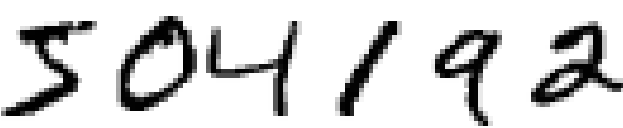
\includegraphics[scale=0.7]{figures/digits}
%\caption{\small \sl Figuren viser tallene 504192. \cite{Nielsen 2019} \label{fig:digits}} 
%\end{center} 
%\end{figure} 

%Menneskets evne til å se er en av de mest fasinerende mirakelene i naturen. Folk flest kan uten anstrengelse gjenkjenne tallene 504192 i figur \ref{fig:digits}. At dette er lett er et under, og ikke minst misledende. In each hemisphere of our brain, humans have a primary visual cortex, also known as V1, containing 140 million neurons, with tens of billions of connections between them. And yet human vision involves not just V1, but an entire series of visual cortices - V2, V3, V4, and V5 - doing progressively more complex image processing. We carry in our heads a supercomputer, tuned by evolution over hundreds of millions of years, and superbly adapted to understand the visual world. Recognizing handwritten digits isn't easy. Rather, we humans are stupendously, astoundingly good at making sense of what our eyes show us. But nearly all that work is done unconsciously. And so we don't usually appreciate how tough a problem our visual systems solve.

%The difficulty of visual pattern recognition becomes apparent if you attempt to write a computer program to recognize digits like those above. What seems easy when we do it ourselves suddenly becomes extremely difficult. Simple intuitions about how we recognize shapes - "a 9 has a loop at the top, and a vertical stroke in the bottom right" - turn out to be not so simple to express algorithmically. When you try to make such rules precise, you quickly get lost in a morass of exceptions and caveats and special cases. It seems hopeless.

%Neural networks approach the problem in a different way. The idea is to take a large number of handwritten digits, known as training examples

\subsection{Tidligere arbeid}

Noen forskere har allerede rukket å anvende ``deep learning'' til å klassifisere fisk fra undervannsvideo. This working note describes the results of CVG Jena Fulda team for the fish recognition task in SeaCLEF 2016. Our method is based on convolutional neural networks applied to object proposals for detection as well as species classification. We are using background subtraction proposals that are filtered by a binary SVM classifier for fish detection and a multiclass SVM for species classification. Both SVM’s utilize CNN features extracted from AlexNet. With this pipeline we achieve a recog- nition precision of 66 \% and a normalized counting score of 58 \% on the provided test dataset. We also show that classification of background subtraction proposals works much better for fish detection than back- ground subtraction on its own. \cite{Jäger m.fl. 2016}

Siddiqui sitt team presenterte i 2017 klassifisering av forskjellige fiskearter i undervannsvideoer ved å bruke en modell  med vekter fra forhåndstrente dype nettverk. Dette automatiske systemet kunne med høy nøyaktighet detektere, tracke og klassifisere fisk og andre marine arter i undervannsvideoer uten menneskelig overvåkning. De oppdaget at typiske maskinsynteknikker fungerer dårlig på undervannsbilder. Bakgrunnen er kompleks og både fasongen og teksturen på de forskjellige fiskeartene kan være svært like. Datadrevne programmer, slik som nevrale nettverk, krever enorme mengder katagorisert data, ellers har de en tendens til å overtilpasse treningsdataen og feiler når den blir gitt testdata som den ikke har sett før, det vil si data som ble utelatt ved treningen. I artikkelen deres  ``Automatic fish species classification in underwater videos'' presenteres state-of-the-art maskinsynsmetoder for fine-grained klassifisering av fiskearter basert på deep learning teknikker. ``Convolutional'' nevrale nettverk, nettverkene som anvendes til bildeklassifisering, ble forhåndstrent på et mye større og mer generelt datasett. Ved å forhåndstrene nettverket på et generelt datasett så kan man bruke mindre treningsdata. SVM ble brukt til å trene nettverket og de oppnådde en nøyaktighet på 94.3 \%. De tropiske fiskeartene ble tatt fra undervannsvideoer fra kysten av vest-Australia. Forskerne mener automatiske klassifiseringssystemer kan brukes til å identifisere fisk fra undervannsvideoer, og at det er et billig alternativ til manuell identifikasjon av fisk. \cite{Siddiqui m.fl. 2017}

I 2018 presenterte Xu og Matzner forskning på deteksjon, tracking og klassifisering av fisk i undervannsvideoer. Undervannsvideoer anvendes til å studere økosystemene i havene og i elver, først og fremst for å drive med miljøforskning. Å observere mengden av liv, samt vanene til fiskene i forskjellige miljø er eksempler på miljøforskning. Optisk video gir detaljert informasjon som mennesker kan forstå, mennesker kan naturlig forstå verden visuelt. Manuell analyse av video tar tid. Å automatisere arbeidet er nødvendig om en har store datamengder, og en ønsker å få arbeidet fullført på en gitt tid på en effektiv måte. Dette kan være nødvendig om en skal gjøre gode avgjørelser som påvirker de marine økosystemene. Maskinsyn og maskinlæring har vist seg å være effektive metoder for å automatisere overvåking. Undervannsbilder er kjent for å være spesielt utfordrende å håndtere. Mengden lys under vann varierer over tid, og mengden lys påvirkes også av avstand fra lyskilder. Det er lite kontrast under vann og bakgrunnen er ofte svært avansert, den består av blant annet flytende vegetasjon. Videre påvirkes bildene av turbidity [1].  Recently, a research tool for studying fish in underwater video was developed by the Fish4Knowledge project [2], and the dataset consisting of mostly coral reef fish were made publicly available.  The web-based software provides researchers with a suite of computer vision methods that can be applied to underwater video for detecting, tracking and \cite{Xu og Matzner 2018}

Salman sitt team viste i 2019 at de kunne måle biomasse automatisk ved å bruke undervannsvideoer og dype nevrale nettverk.  Et slikt system må takle varierende lysstyrke, vinkelen fiskene sees fra, forskjellige havbunn strukturer, bevegelser i vegetasjon i bakgrunnen og forskjellige former og teksturer mellom fiskearter. De anvendte en Region-Based Convolutional Neural Network, et R-CNN, som er en state-of-the-art maskinlæringsteknikk, et alternativ til YOLO. Teknologien anvendes til objektdeteksjon, den gir informasjon om hvor i et bilde forskjellige objekter er samt hvor mange det er av de forskjellige objektene. De trente et nevralt nettverk, we employ a novel approach to utilize motion information of fish in videos via background subtraction and optical flow, and subsequently combine the outcomes with the raw image to generate fish-dependent candidate regions. We use two benchmark datasets extracted from a large Fish4Knowledge underwater video repository, Complex Scenes dataset and the LifeCLEF 2015 fish dataset to validate the effectiveness of our hybrid approach. De oppnådde en deteksjonsnøyaktighet (F-Score) på 87.44 \% og 80.02 \% respectively on these datasets, which advocate the utilization of our approach for fish detection task. Monitoring the effect of preventive and recovery measures requires the estimation of fish biomass, and abundances by sampling their populations in water bodies like lakes, rivers and oceans on a regular basis (Jennings and Kaiser, 1998). This requires observation of the interaction of different fish species with changing environmental conditions. This is an essential process, especially in those regions of the world where certain species of fish are either threatened or at the risk of extinction due to habitat loss and modification, industrial pollution, deforestation, climate change, and commercial overfishing (Tanzer et al., 2015). There is a well-established and increasing interest in using nondestructive fish sampling techniques by marine biologists and conservationists (McLaren et al., 2015). Underwater video-based fish detection approaches have been used to achieve nondestructive and repeated sampling for many years \cite{Salman m.fl. 2019}

I 2020 så tok Cui sitt team undervannsrobotikk videre i forskningsartikkelen deres ``Fish Detection Using Deep Learning''. The ocean is full of mystery and the underwater exploration has always been an exciting topic. Nowadays, robotics has been widely adopted into our daily lives. The AUV is one type of robot, which is gaining more and more attention [1, 2]. It must be equipped with a sophisticate onboard computer, Inertial Measurement Unit (IMU), and other sensors to be able to support a preprogrammed navigation system [1]. Authors have experience on design and function of an AUV [3, 4] for competitions. The AUV, as shown in Figure 1, is featured with an i7-based industrial motherboard plus an ARM microcontroller. Detail hardware layout and mechanical balancing scheme are introduced in [3, 4]. It passed the qualification and became one of the eleven finalists at the 2017 IEEE Singapore AUV Challenge [5]. This competition was hosted in a swimming pool of clear water. The tasks did not need a high-resolution camera, so the major processor was not chosen to be of high performance. After this the AUV retired from the competition, authors realized it was time to revise the system to conquer real life tasks. As of now, most of the robot control platforms were shifting to Systems-On-Chip (SOC) [6, 7]. To move forward and add more functionalities to the AUV, one goal is to switch from a clear swimming pool environment to a real ocean water condition. Therefore, the hardware has to be upgraded to high resolution digital camera along with a powerful onboard computer, such as NVIDIA JETSON AGX XAVIER development board. \cite{Cui m.fl. 2020}

%\subsection{Perceptron}

%\subsection{Sigmoid neurons}